\documentclass{beamer}

\mode<presentation>
{
  \usetheme{Montpellier}
  \usecolortheme{beaver}
  \setbeamercovered{transparent}
}

\usepackage[english]{babel}
\usepackage[latin1]{inputenc}
\usepackage{times}
\usepackage[T1]{fontenc} 
% Or whatever. Note that the encoding and the font should match. If T1
% does not look nice, try deleting the line with the fontenc.
\usepackage{amsmath}
\newcommand{\linespace}{\vskip 0.25cm}

\definecolor{MyForestGreen}{rgb}{0,0.7,0} 
\newcommand{\tableemph}[1]{{#1}}
\newcommand{\tablewin}[1]{\tableemph{#1}}
\newcommand{\tablemid}[1]{\tableemph{#1}}
\newcommand{\tablelose}[1]{\tableemph{#1}}

\definecolor{MyLightGray}{rgb}{0.6,0.6,0.6}
\newcommand{\tabletie}[1]{\color{MyLightGray} {#1}}

% The text in square brackets is the short version of your title and will be used in the
% header/footer depending on your theme.
\title[Thermal Interaction In SAR]{Thermal Interaction in \\ Spatial Augmented Reality}

% Sub-titles are optional - uncomment and edit the next line if you want one.
% \subtitle{Why does sub-tree crossover work?} 

% The text in square brackets is the short version of your name(s) and will be used in the
% header/footer depending on your theme.
\author[YaDeau]{Justin Brennen YaDeau}

% The text in square brackets is the short version of your institution and will be used in the
% header/footer depending on your theme.
\institute[U of Minn, Morris]
{
  Division of Science and Mathematics \\
  University of Minnesota, Morris \\
  Morris, Minnesota, USA
}

% The text in square brackets is the short version of the date if you need that.
\date[December '15] % (optional)
{5 December 2015}

% Delete this, if you do not want the table of contents to pop up at
% the beginning of each subsection:
\AtBeginSection[]
{
  \begin{frame}<beamer>
    \frametitle{Outline}
    \tableofcontents[currentsection, hideothersubsections]
  \end{frame}
}

\begin{document}

\begin{frame}
  \titlepage
\end{frame}

% For a 20-25 minute senior seminar talk you probably want something like:
% - Two or three major sections (other than the summary).
% - At *most* three subsections per section.
% - Talk about 30s to 2min per frame. So there should probably be between
%   15 and 30 frames, all told.

%\section*{Overview}

%\subsection*{Background}

%\begin{frame}
%  \frametitle{Background}
  
%  \begin{columns}
%  \begin{column}{0.6\textwidth}
%  \begin{itemize}
%  	\item Virtual Reality
%	\item Augmented Reality
%	\item Spatial Augmented reality
%	\item 6DOF
%  \end{itemize}
%  \end{column}
%  \end{columns}
%\end{frame}

\subsection*{Outline}
\begin{frame}
  \frametitle{Outline}
  \tableofcontents[hideallsubsections]
\end{frame}

\section[Mobile Thermal Interaction]{Thermal interaction with mobile devices}

\subsection{Applications}

\begin{frame}
	\frametitle{Applications}
	Applications that use thermal imaging with mobile technology 
	\begin{itemize}
		\item "Spray on" GUIs
		\item Augmented floor plans
	\end{itemize}
\end{frame}

\begin{frame}
	\frametitle{"Spray on" GUIs}
	
	\begin{columns}
	\begin{column}{0.45\textwidth}
	\begin{itemize}
		\item What are Spray on GUIs?  
		\item Usability
	\end{itemize}
		
	\end{column}
	\begin{column}{0.55\textwidth}
	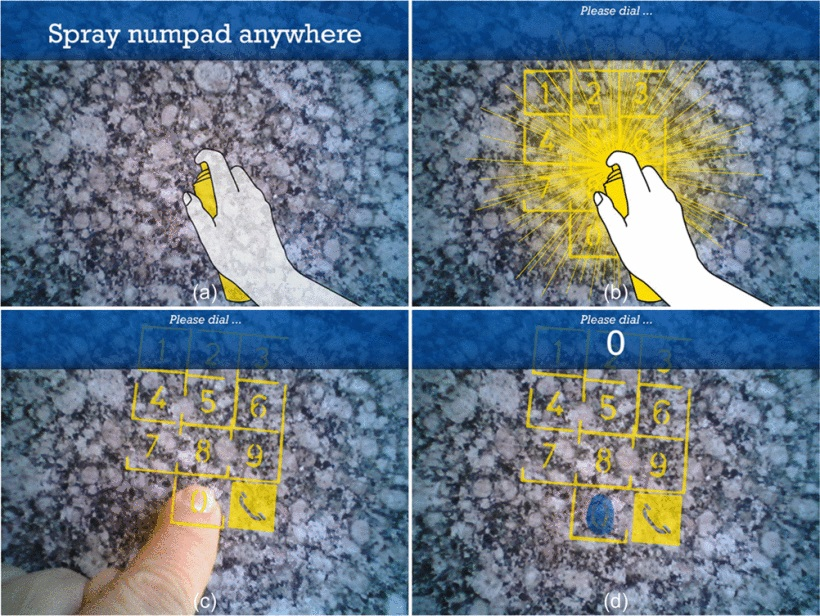
\includegraphics[width=\textwidth]{../Sample_paper/images/numpad}
	\end{column}
	\end{columns}
\end{frame}

%\begin{frame}
%	\frametitle{Augmented floor plans}
%	\begin{columns}
%	\begin{column}{0.45\textwidth}
%	\begin{itemize}
%		\item 
%	\end{itemize}
%	\end{column}
%	\begin{column}{0.55\textwidth}
%	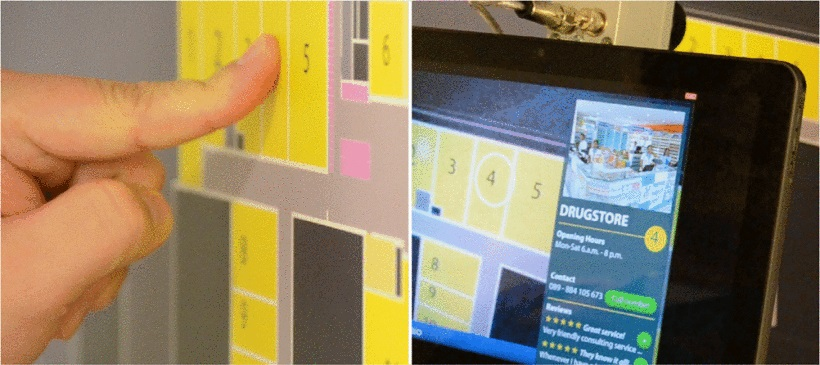
\includegraphics[width=\textwidth]{images/AugmentedFloorPlans}
%	\end{column}
%	\end{columns}
	
%\end{frame}

\section[Using SAR for 3D data visualization]{Using SAR for 3D data visualization}
\begin{frame}
\frametitle{Using SAR for 3D data visualization}
\end{frame}


\section[Conclusions]{Conclusions}
\begin{frame}
\frametitle{Conclusions}
\end{frame}

\begin{frame}
	\frametitle{Thanks!}
	
	Thank you for your time and attention!
		
	\linespace
	\linespace
	
	Contact:  
	\begin{itemize}
		\item \texttt{yadea003@morris.umn.edu}
	\end{itemize}
	
	\linespace
	\linespace
	
	\begin{center}
	{\huge Any Questions?}
	\end{center}
\end{frame}

\end{document}


